% !TEX root = ./proj_report.tex
\graphicspath{{mehul_pics/}}% Set graphics path location

\section{Image Filtering}

Blurred images are modeled as the true image convolved with a point spread function (PSF) with additive noise. The point spread function that convolves the true image is generally a property associated with the optics that has contributed to the blur while noise can be due to poor/excessive illumination, quantization errors and other sources. In this report terms PSF and kernel will be used interchangeably. Mathematically, a blurry image can be represented as follows

\begin{equation}
v(m,n)= h(m,n) \star u(m,n) + \eta(m,n)
\end{equation}
where, $u(m,n)$ is the true image, $h(m,n)$ is the PSF, $\eta(m,n)$ is the additive noise and $v(m,n)$ is the blurry image. Image sharpening involves calculating an estimate of the true image $\hat{u}(m,n)$ using filters.

\begin{equation}
\hat{u}(m,n)= g(m,n) \star v(m,n)
\end{equation}
Where $g(m,n)$ is a kernel computed by the filter using some knowledge of the PSF that caused the blur and an estimate of the signal to noise ratio.

\subsection{Filter kernels}
The choice of filter is very important in image restoration and for the retrieval of image characteristics. This part of the project aims to study and compare different filters based on the kernel shape, as well as visual confirmation. The scope of this project encompasses the use of disk, Gaussian, and motion kernels to generate and guess the source of blur.\\
\noindent The filters use for this study are: 
\begin{enumerate}
\item Inverse and Pseudo-inverse
\item Wiener
\item Geometric mean
\item Constrained least squares
\end{enumerate} 
Mathematical formulation of these filters have been presented in the Appendix  and will not be discussed here. 
\subsection{Train Image: Supersonic flow around a sphere}
In this simulated motion blur, the train image was procured from Van Dyke's Album of Fluid Motion~\cite{VanDyke:1982}, and depicts the formation of shock around a sphere Mach no. of  3. This image was blurred using a motion kernel and was supplied Gaussian white additive noise. This image was sharpened with all the previously mentioned filters. The blur kernel was used as the initial guess PSF for the filters, and the noise variance was set to $10^{-5}$. 
Through this analysis it was concluded that the Wiener filter performed the best at reconstructing the true optical kernel for this image, this conclusion was reached by comparing each of the filter approximated kernels with the kernel used to blur the image. The metric used for this comparison was the 2-norm of the difference between the 2D projections of the filter obtained kernel and the kernel used to blur the image. A plot of the kernels is shown in Figure~\ref{fig:sph_kernels}.

\begin{figure}[H]
  \centering
                \centering
                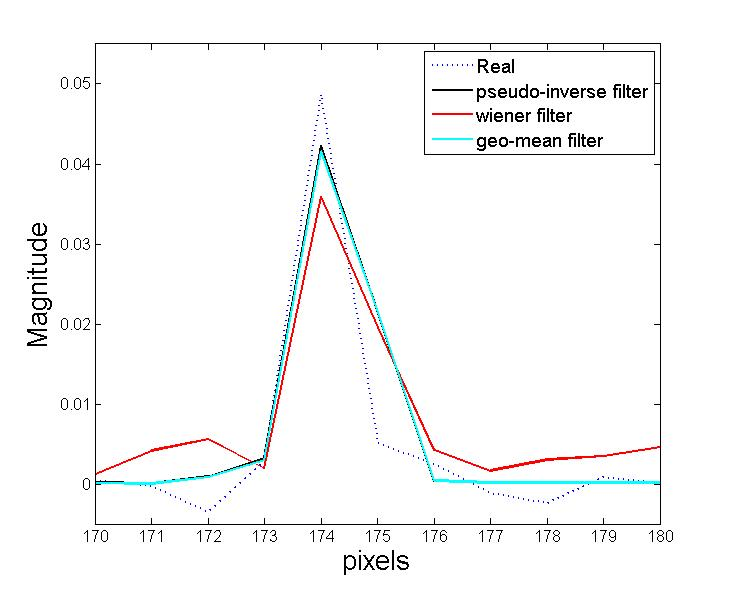
\includegraphics[width=.4\textwidth]{kernel_motion.jpg}
                \caption{Kernel comparison for motion induced blur on a supersonic sphere}
 \label{fig:sph_kernels}
\end{figure}

Although this approach has proven to be very useful for the study of training images, the use of it with real blurred images is very challenging. Some of the draw backs encountered with this approach is its dependence on a-priory knowledge of the blur cause, as well as noise sources and strengths. 
\subsection{Real Image: Barn and Barrels}
To test this approach with real blurred images, two images of the same source have been captured, one clear and one out-of-focus. The captured images are shown on Figure~\ref{fig:barrels}. With the use of a de-convolution between captured clear and out-of-focus images, the true kernel was obtained. To reduce the effect of noise in the kernel, both images were split in multiple parts, each pair was used to obtain a kernel independently, and then averaged to obtain an approximation of the true kernel were noise is reduced. A similar analysis as the one done for the sphere was performed, and a comparison between the true and filter obtained kernels can be seen in Figure~\ref{fig:true_kernel}.

\begin{figure}
        \centering
        \begin{subfigure}[b]{0.32\textwidth}
                \centering
                \includegraphics[width=\textwidth]{DSC_0517.jpg}
                \caption{Clear image}
                
        \end{subfigure}
        \hspace{1.5cm}
        \begin{subfigure}[b]{0.32\textwidth}
                \centering
                \includegraphics[width=\textwidth]{DSC_0518.jpg}
                \caption{Image Out-of-focus} 
        \end{subfigure}
\caption{Experimental images}
\label{fig:barrels}
\end{figure}

\begin{figure}[H]

  \centering
                \centering
                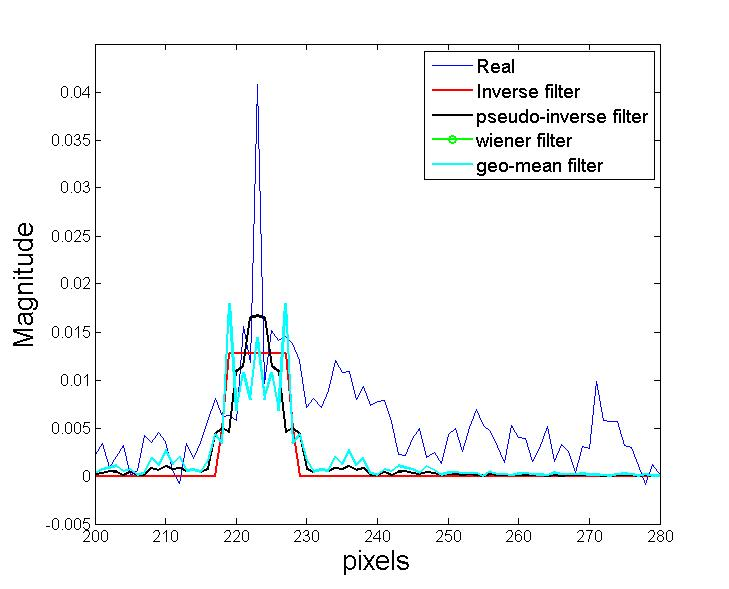
\includegraphics[width=.4\textwidth]{true_kernel.jpg}
                \caption{All previously mentioned filters have been used to approximate the true kernel. The blur PSF used as the initial condition for the filtering process is "disk". Variance of the additive noise is set to $10^{-3.5}$ }
                \label{fig:true_kernel}
\end{figure}

As can be seen from Figure~\ref{fig:true_kernel}, the approximations for the kernel are not very good, and without knowing the true cause of the blur, it is very challenging and time consuming to find a filter that will be able to sharpen the image. Due to the presence of undetermined noise, we can't just use a simple norm to determine the effectiveness of a filter type anymore. To be able to deal with real blurred images sharpness metrics are required.
\newpage